
\graphicspath{{./fig1/}}

\section{V-Sphereとソルバークラス}
\label{sec:1.1}
複数の物理ソルバを連成したマルチフィジックス解析では,複数ソルバの実行制御・管理の問題が顕在化している.物理シュミレーションの数値解法は,各々の現象に対して効率のよい固有の解法として発展し,専門性の強い研究領域を形成している.一人の研究者で全ての現象解析をカバーすることは難しいため,連成解析のシステム開発にあたり,研究者間のコラボレーションを促進する仕組みには大きな期待が寄せられている.具体的には,プログラム開発のガイドライン,あるいは共通機能を持つフレームワークを利用することにより,開発効率やプログラムの品質の向上を図ることができる.特に,大規模なソフトウェア,複数のプログラマによる協同作業の場合には,作業効率やメンテナンス性の点からはこれらの仕組みが必須である.

プログラムの開発支援と実行管理の問題点に対して,著者らは物理シミュレーションのひな型の提供と複数のソルバーコードを管理し,選択・連成実行可能なアプリケーションの機能を持つオブジェクト指向フレームワークV-Sphereを提案している~\cite{ono:V-SphereJSCES, ono:V-SphereACS18, ono:SphereParCFD08}.
このフレームワークは,オブジェクト指向技術の積極的な利用により,非定常/定常物理シミュレーションのソフトウェア構造の標準化・統一化を推進している.また,アプリケーションの開発効率化・高品質化・メンテナンス性の向上に貢献し,先端シミュレーション技術の迅速なパッケージングが期待できる.

V-Sphere\index{V-Sphere}は,非定常物理シミュレーションのフレームワークとして設計されている.
V-Sphereフレームワークは,\textbf{図\ref{fig:V-Sphere_framework}}に示す様々なライブラリ機能と\textbf{図\ref{fig:Control_structure}}に示す非定常物理現象のシミュレータに共通する制御構造をソルバー開発者に提供する.
つまり,時間的に変化する物理現象の解析プログラムはどれも同様に記述できる点に着目し,処理の大まかな流れ(前処理,本計算,後処理の3つのステージ)を規定し,共通機能を抽出し,APIとしてまとめている.
制御構造はSklSolverBase\index{SklSolverBase}クラスに内包されており,開発者はこのソルバー基底クラスを継承したクラスを作成し,この派生クラスにユーザ関数・サブルーチンをクラスメソッドとして実装することによりプログラムを作成する.
また,通常の意味でのサブルーチンも多く用意し,計算パラメータなどの入力データ,計算結果の入出力などの機能を提供している.
これらの利用により,ソルバ開発者にとって本質的でないプログラミングを減らし,開発の効率化が期待できる.
システムの実装はオブジェクト指向に基づきC++で記述されているが,従来資産の移行,物理コードの開発者がCやFortran言語を使い慣れていることを考慮し,プログラミングモデルとしては手続き型言語の記述を基本としている.具体的には,Fortran/C言語へのインタフェースを備えている.

\begin{figure}[htbp]
\begin{center}
\includegraphics[width=12cm,clip]{V-Sphere_framework.eps}
\end{center}
\caption{V-Sphere frameworkのブロック図.V-Sphereは様々な機能,たとえば並列ライブラリ,ファイル入出力,XML記述によるパラメータハンドリングなどを内包する.}
\label{fig:V-Sphere_framework}
\end{figure}

\begin{figure}[htbp]
  \begin{minipage}{.47\textwidth}
  	\begin{center}
  	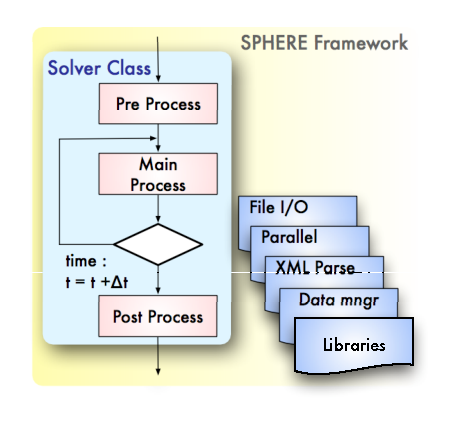
\includegraphics[width=8cm,clip]{Sphere_Control.eps}
  	\end{center}
  	\caption{V-Sphereの制御構造.プリ,メイン,ポストの処理プロセスが組み込まれており,提供されるライブラリ機能を用いてソルバークラスを構築する.}
	\label{fig:Control_structure}
  \end{minipage} \hfill
  \begin{minipage}{.47\textwidth}
	\begin{center}
  	\includegraphics[width=7.5cm,clip]{CubeFamilies.eps}
  	\end{center}
  	\caption{差分プログラミングによるソルバークラスの開発.SklSolverBaseクラスから派生させて目的のソルバークラスを作成する.ソルバークラスC3D-AはC3Dから派生しており,必要な機能だけが追加でプログラミングされる.また,必要に応じて,ユーザが定義したクラスライブラリに共通機能をまとめて利用できる.}
  	\label{fig:DerivedSolvers}
  \end{minipage}
  \vspace*{2mm}
\end{figure}

V-Sphereは,非定常物理シミュレーションのソルバー開発を支援する抽象度の高い汎用的なプログラム部品群をクラスライブラリの形式で提供する.
それらのうち主要なクラスはSklSolverBaseクラスに既に組み込まれている.
例えば,ファイル入出力,ソルバー制御・物理・境界条件パラメータの読み込みと保持,ボクセルデータの前処理,境界条件の制御などの機能があり,プログラムに対するユーザーインターフェイスを規定する役割を果たす.

V-Sphereの機能を用いて作成したアプリケーションはソルバークラスとしてV-Sphere自身に登録することができ,登録されたソルバークラス群は共通のユーザインターフェイスを備えたアプリケーションとして振る舞う.これはエンドユーザから見ると,利用しやすいアプリケーション群と認識されるであろう.
V-Sphere では,\textbf{図\ref{fig:DerivedSolvers}}に示すようにSklクラス,SklBase\index{SklBase}クラス,およびSklSolverBaseクラスを提供する.SklSolverBaseクラスからSklSolverFBクラスとSklSolverStructクラスが派生し,さらにSklSolverFBクラスからは各ソルバクラスが派生している.
\textbf{図\ref{fig:DerivedSolvers}}には,ソルバークラスC3Dから派生した2つのソルバークラスを示している.
これらの2つのソルバークラスC3D-A, C3D-Bは,基本的な機能はC3Dクラスの機能を持つが,例えば,シミュレートする物理現象や形状近似度,変数配置などが異なるソルバーと考えることができる.
異なるソルバーであっても,同じ基底クラスを利用してアプリケーションを開発することによって,ユーザーインターフェイスが統一されたアプリケーションとして構築することができる.

具体的なアプリケーションを構築する場合には,V-Sphereが提供する基本的な機能部品を用いて,より具体的な機能を構成する必要がある.
つまり,ソルバークラスの詳細な処理の記述はユーザに任されている.
そこで,適用範囲を限定しながらもある程度の汎用性をもつクラスを作成する必要がある.
これには,二種類の方法がある.
\textbf{図\ref{fig:V-Sphere_framework}}において,ユーザー定義クラス\index{ゆーざーていぎくらす@ユーザー定義クラス}やユーザー定義基底クラス\index{ゆーざーていぎきていくらす@ユーザー定義基底クラス}がそれに相当する.
ユーザー定義クラスは,文字通り,ユーザーが作成したクラスである.ユーザー定義クラスは通常のオブジェクト指向プログラミングに従い,SklSolverBaseクラスの中でインスタンスして利用することができる.
一方,ユーザー定義基底クラスは,SklSolverBaseクラスを派生させたクラスで,これからさらに派生させたソルバークラスでの利用を想定している.
つまり,ソルバー開発者はユーザー定義基底クラスを派生させて具体的なソルバークラスを作成する.
V-Sphereを用いたコード開発では,両方のアプローチを利用している.

シミュレーションプログラムの利用価値を高めるためには,コードのポータビリティを始めとして,開発の効率化支援と共にメンテナンス性や利用環境なども考慮する必要がある.
この観点から,V-Sphereは開発者とエンドユーザーの双方に利便性を提供する.

\begin{itemize}
\item 開発の効率化\\
フレームワークの利用により,上位概念でプログラミングができる.つまり,アプリケーション開発者はアルゴリズムの記述に専念でき,またプログラムのメンテナンスが簡単になる.
他方,デメリットとしてはソルバー開発者に,プログラム・データ構造やコーディングの作法を強制する面がある.
\item エンドユーザーに対するインターフェイスの統一化\\
利用するソルバーが異なってもアプリケーションの振る舞いは同様であるので,アプリケーション導入時のハードルは低くなる.
\end{itemize}

大規模な解析を実施する観点からは,並列化が必須となってくる.
V-Sphereは,並列化も含めシミュレーションプログラム開発の効率的な開発環境を提供すること,マルチフィジックス問題を扱うことも視野に入れ複数のコードの実行管理を行うことを視野に入れている.
逐次コードから並列コードへの拡張については,簡単なライブラリコールにより領域分割型の並列化に対応できるように工夫され,高い並列化性能がでることを確認している.

%
\section{ソルバークラス}
\label{sec:1.2}
V-Sphereに移植されたソルバークラスを\textbf{表\ref{tbl:solverclass}}に示す\footnote{\today 現在}.FBクラスは,具体的な流体ソルバークラスを開発するために使うクラス群であり,単体では動作しない.

\begin{table}[htdp]
\caption{V-Sphereで稼働するソルバークラス}
\small
\begin{center}
\begin{tabular}{ll} \toprule
Solver Class & Solverの説明\\ \midrule
CBC & 直交系の単層流三次元非圧縮非定ソルバークラス\\
FB & 流体解析に用いる基本パッケージクラス\\ \bottomrule
\end{tabular}
\end{center}
\label{tbl:solverclass}
\end{table}

%
\section{V-Sphereユーザーガイドの構成}
\label{sec:1.3}
本ユーザーガイドの構成は以下のようになっている.2章ではMPI通信ライブラリ,V-Sphereの環境設定,およびソルバークラスのインストールについて詳細に記述している.
